     Son consideradas figuras: gráficos, diagramas, láminas, fotografías,
esquemas de cualquier naturaleza, dibujos, planos, organigramas, flujogramas,
cuadros y tablas tanto en color como blanco y negro...

\subsection{Presentación Gráfica}
       
Un ejemplo es la figura~\ref{fig:pucv}....


\begin{figure}[!htbp]
\begin{center}
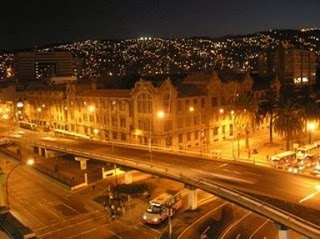
\includegraphics[width=0.6\linewidth]{Images/pucv.jpg} 
\caption{Edificio PUCV.}\label{fig:pucv}
\end{center}
\end{figure}